% reducesymm/elton/Arxiv_paper/PCF.tex      pdflatex ECHG24; biber ECHG24
% Predrag separated out to minimize conflicts    2025-01-10 

\section{{\PCf}}
\label{s:PCF}

\subsection{The Navier-Stokes equations}
\label{s:NS}
 The underlying equations
that govern the motion of \pCf\ are the {\NSe}s,
along with boundary conditions. The boundary conditions for \pCf\ in the $x$
and $z$ directions are periodic,
 $ \bu(x, y, z) = \bu(x+L_x, y, z) =
\bu(x, y, z + L_z) $.
 In the $y$ direction,
 $\bu = (1,0,0)$ at $\bx = (0,1,0)$ and $\bu = (-1,0,0)$ at $\bx =
 (0,-1,0)$.

 The fluid is taken to be incompressible, so in this case the
 {\NSe}s are
 \beq
 \frac{\partial \bu}{\partial t} + (\bu \cdot \nabla)\bu = -\nabla p + \frac{1}{Re} \nabla^{2} \bu
    \,,\qquad
\nabla \cdot \bu  = 0 \,. \label{eqn:NavierStokes} \eeq 



For an Eulerian equilibrium velocity field that is not changing in time, 
the first equation in \refeq{eqn:NavierStokes} simplifies to 
\beq
 (\bu \cdot \nabla)\bu = -\nabla p + \frac{1}{Re} \nabla^{2} \bu
    \,, 
\ee{eqn:NavierStokes2}
 
The Reynolds number parameter $\Reynolds$, which gives a measure of fluid 
viscosity and degree to which fluid motion may become turbulent, is given 
by 
\beq Re = \frac{\overline{u}L}{\nu} 
\eeq 
where $\overline{u}$ is the average fluid velocity and $L$ is the 
characteristic length. Thus the form of the {\NSe}s and boundary 
conditions make use of rescaling to use non-dimensionalized variables. We 
use $\Reynolds = 400$, in the regime of transitional turbulence, for the 
\pCf\ simulations throughout the text. 

For computational purposes, it is easier to work with a velocity field  that
represents the {difference} from the laminar flow. 
So we can break up the total field into two components: $\butot =
y \hat{\bf x} + \bu$. Here $y \hat{\bf x}$ is the laminar velocity
field and $\bu$ is then the difference between the total velocity and
laminar. Substitute $y \hat{\bf x} + \bu$ for $\bu$ in the
nondimensionalized {\NSe}s above to get
\beq
    \frac{\partial \bu}{\partial t}
    + y  \frac{\partial \bu}{\partial x}
    + v \, \hat{\bf x}
    + \bu \cdot \bnabla \bu
=
    - \bnabla p
    + \frac{1}{\Reynolds}
        \lapl \bu  \,, \quad \nabla \cdot \bu = 0
\,,
\ee{NavStokesDiff}
with boundary conditions $\bu = 0 $ at $y \pm 1$.  Having 
Dirichlet boundary conditions on $\bu$ makes the analysis much easier, 
since the set of allowable velocity fields (those fields that satisfy 
incompressibility and boundary conditions) forms a vector space. The 
equilibrium velocity fields we study start from $\bu$ which satisfies 
\refeq{NavStokesDiff}, and we may then add back the laminar part of the 
flow to produce physical fluid trajectories. 

This study is conducted at $\Reynolds = 400$ in the 
small aspect-ratio cell \citep{GHCW07,HGC08}
\bea
\bNarrow~  &=&       [2\upi/1.14, 2, 2\upi/2.5]
    \continue
           &\approx& [5.51, 2, 2.51]
    \continue
           &\approx& [190, 68, 86] \;\;\; \mbox{wall units}
\label{cellNarrow}
\eea
where the wall units are in relation to a mean shear rate of $\langle
\partial u/ \partial y \rangle = 2.9$ in non-dimensionalized units
computed for a large aspect-ratio simulation at $\Reynolds = 400$.
Empirically, at this Reynolds number the \bNarrow\ cell 
exhibits only short-lived transient
turbulence \citep{GHCW07}. The $z$ length scale $L_z = 4 \upi/5$
of \bNarrow\ was chosen as a compromise between the $L_z = 6 \upi/5$ of
\bNarrow\ and its first harmonic $L_z/2 = 3 \upi/5$ \citep{W02}.
Unless stated otherwise, all calculations
are carried out for $\Re = 400$ and the $\bNarrow$ cell. In the notation
of this paper, the solutions presented in\rf{N90} have wavenumbers
$(\alpha, \gamma) = (0.8, 1.5)$ and fit in the cell $[2 \upi/0.8, 2,
2\upi/1.5] \approx [7.85, 2, 4.18]$.%


%% PC 2024-12-20 copied from n00bs.tex  2009-06-16
\begin{figure}
\centering
{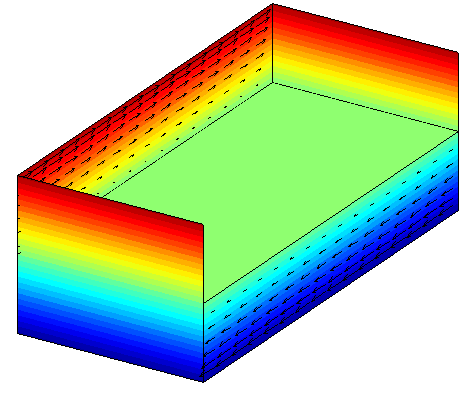
\includegraphics[width=0.31\textwidth]{EQ0}} \hskip -30ex \tEQzero \hskip 25ex
%{\includegraphics[width=0.31\textwidth]{EQ1}} \hskip -30ex \tLB \hskip 25ex
{\includegraphics[width=0.31\textwidth]{EQ2}} \hskip -30ex \tEQtwo \hskip 25ex ~
%{\includegraphics[width=0.31\textwidth]{EQ3}} \hskip -30ex \tNNB    \hskip 25ex
%{\includegraphics[width=0.31\textwidth]{EQ4x}} \hskip -30ex \tNB     \hskip 25ex
%{\includegraphics[width=0.31\textwidth]{EQ5}} \hskip -30ex \tEQfive \hskip 25ex ~
{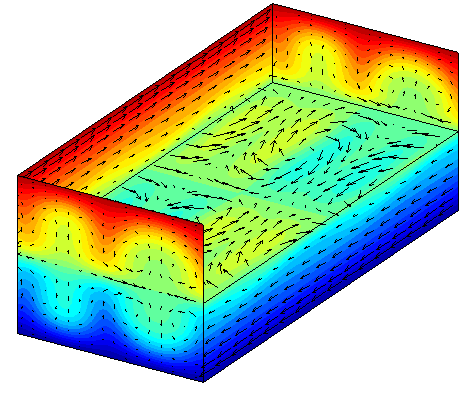
\includegraphics[width=0.31\textwidth]{EQ8}} \hskip -30ex \tEQeight \hskip 25ex ~
%%                              was    {EQ8xz}
%\\
%{\includegraphics[width=0.31\textwidth]{uEQ6Re330box}} \hskip -30ex \tEQsix   \hskip 25ex
%{\includegraphics[width=0.31\textwidth]{EQ6}} \hskip -30ex \tEQsix   \hskip 25ex
%{\includegraphics[width=0.31\textwidth]{EQ7}} \hskip -30ex \tEQsev   \hskip 25ex
%{\includegraphics[width=0.31\textwidth]{EQ9}}  \hskip -30ex \tEQnine \hskip 25ex
%{\includegraphics[width=0.31\textwidth]{EQ10}} \hskip -30ex \tEQten  \hskip 25ex
%{\includegraphics[width=0.31\textwidth]{EQ11}} \hskip -30ex \tEQelev \hskip 25ex ~
    \caption[$3D$ space plots of \tEQtwo\ and \tEQeight.]{
\tEQzero, \tEQtwo\ and \tEQeight\ Eulerian equilibrium solutions of {\pCf} in 
$\bNarrow = [2\upi/1.14, 2, 2\upi/2.5]$ at $Re = 400$. 
The heat map color indicates
the streamwise ($u$, or $x$ direction) velocity of the fluid:
{red} shows fluid moving at $u=+1$,
{blue}, at $u=-1$.
The heat map color as a function of $u$ is indicated
by the laminar {\eqv}, the front face of the
laminar solution \tEQzero, $u(y) = y$, serving as a reference.
From \citet{HGC08}.
    }
\label{f:eqbaboxes}
\end{figure}

\subsection{Computation of trajectories from Eulerian equilibrium velocity fields}
\label{s:channelflow}

 In order to integrate streamlines of {\pCf}
and follow the paths of tracer particles, it is first
necessary to have numerically accurate \eqv\ $3D$-velocity fields.

The starting point for this task is to obtain the necessary data sets for 
evaluating velocity field values for a given \eqv, e.g. the equilibria 
as shown in \reffig{f:eqbaboxes}. These are made available at the website 
{\tt Channelflow.org} \citep{channelflow}. The data obtained 
\citep{channelflowDat} stores the spectral coefficients $\mathbf{\hat{u}}$ 
of the expansion of a velocity field $\mathbf{u(x)}$ satisfying \refeq{NavStokesDiff}. The form of the 
expansion is 
\begin{equation}
 \mathbf{u(x)} = \sum_{m_{y}=0}^{M_{y}-1}\sum_{m_{x}=0}^{M_{x}-1}\sum_{m_{z}=0}^{M_{z}-1}
 {\mathbf{\hat{u}}_{m_{x},m_{y},m_{z}} \bar{T}_{m_{y}}(y)e^{2\pi i(k_{x}x/L_{x} + k_{z}z/L_{z})}}
\label{eqn:spectralsum}
 \end{equation}

The $\bar{T}(y)$'s are Chebyshev polynomials defined on the interval 
[-1,1]. For a given velocity field expansion, the 
upper bounds on the sums are known from the geometry, and the $k$'s are 
related to the $m$'s through the following relations: 
 \beq 
k_{x} = \left \{ 
\begin{array}{l}
m_{x} \hspace{20 mm} 0 \leq m_{x} \leq M_{x}/2   \\
m_{x} - M_{x} \hspace{10 mm} M_{x} < m_{x} < M_{x}  \\
\end{array}  \right.
\eeq 
\beq k_{z} = m_{z} \hspace{10 mm} 0 \leq m_{z} < M_{z}
\,.
\eeq
Hence, with a knowledge of the spectral coefficients we can compute 
$\mathbf{u(x)}$ by evaluating this sum at a particular $\bx = (x,y,z)$. 

Various internal functions within {\tt Channelflow.org} have been written 
to compute $\bu$ on a set of gridpoints. It is possible, by interpolation 
of the velocity fields on these gridpoint values, to integrate a 
trajectory with great computational speed. However this will not be 
nearly as accurate as evaluating the sum \refeq{eqn:spectralsum} 
directly. So we evaluate \refeq{eqn:spectralsum} to give the exact 
velocity field at every point along a trajectory, adding back the laminar part of the flow. We are able to perform 
these computations in Matlab with enough speed to compute many tracer 
particle trajectories within an Eulerian equilibrium velocity for an adequate 
length of time to study the flow dynamics.  


\subsection{Symmetries of {\pCf}}
\label{s:PCF_symm}

As part of our theoretical analysis of trajectories of fluid particles 
within an Eulerian equilibrium velocity field, it will be critical to use and 
understand the symmetries involved in the special geometry of {\pCf}. 
Thus we take a quick detour to discuss these symmetries from a 
group-theoretic perspective. We focus on the symmetries relevant to the 
Eulerian equilibria studied in this work; additional details are provided in 
\citet{HalcrowThesis}. 

\PCf\ is invariant under two reflections $\sigma_1,\sigma_2$ and a
continuous two-parameter group of translations $\tau(\shift_x, \shift_z)$:
\bea
\sigma_1 \, [u,v,w](x,y,z) &=& [u, v,-w](x,y,-z) \continue
\sigma_2 \, [u,v,w](x,y,z) &=& [-u,-v,w](-x,-y,z)  \label{reflSfit1}\\
\tau(\shift_x, \shift_z)[u,v,w](x,y,z) &=& [u,v,w](x+\shift_x,y,z+\shift_z) \nnu\,.
\eea
The \NSe s and boundary conditions are invariant for any symmetry $s$
in the group generated by these elements:
$\partial (s \bu) / \partial t = s (\partial \bu / \partial t)$.

The {\pC} symmetries can be interpreted geometrically in the space of
fluid velocity fields. Let $\bbU$ be the space of
square-integrable, real-valued velocity fields that satisfy the kinematic
conditions of \pCf:
\bea
 \bbU  &=& \{\bu \in L^2(\Omega) \; | \; \grad \cdot \bu = 0,
               \; \bu(x, \pm 1, z) = 0, 
 %\notag  
 \continue
       &\phantom{=}&  {} \qquad \qquad \qquad \; \; %\mbox{and }
          \bu(x, y, z) = \bu(x+L_x, y, z) = \bu(x, y, z + L_z)\}  
\,.
\nnu
\eea
The continuous symmetry $\tau(\shift_x, \shift_z)$ maps each state
$\bu \in \bbU$ to a $2D$ torus of states with identical dynamic
behavior. This torus in turn is mapped to four equivalent tori by
the subgroup $\{1,\sigma_1,\sigma_2, \sigma_1 \sigma_2\}$. In
general a given state in $\bbU$ has four $2D$ tori of dynamically
equivalent states.

Most of the Eulerian \eqva\ that are currently known for \pCf\
are invariant under the `shift-reflect' symmetry
$s_1 = \tau(L_x/2,0) \, \sigma_1$ and the `shift-rotate' symmetry
$s_2 = \tau(L_x/2,L_z/2) \, \sigma_2$.  These symmetries form a group
\beq
S = \{1, s_1, s_2, s_3\}, \qquad s_3 = s_1 s_2, 
\eeq
which is isomorphic to the Abelian dihedral group $D_2$, and is a 
subgroup of a larger group generated by {\pC} symmetries. The 
group acts on velocity fields as: 
\bea
s_1 \, [u, v, w](x,y,z) &=& [u, v, -w](x+L_x/2,\, y,\, -z) \continue 
s_2 \, [u, v, w](x,y,z) &=& [-u, -v, w](-x+L_x/2,\,-y,\,z+L_z/2) \label{shiftRot} \\
s_3 \, [u, v, w](x,y,z) &=& [-u,-v,-w](-x,\, -y,\, -z+L_z/2)  \nnu 
\,
\eea

We denote the $S$-invariant subspace of states invariant under
symmetries \refeq{shiftRot} by
\bea
\bbUsymm  &=& \{\bu \in \bbU  \: | \;
              s_j \bu = \bu\,, \;\;  s_j \in S \}
              % \bu = \frac{1}{4} (1 + s_1 + s_2 + s_3)\,\bu \}
\,,
\label{symmSubspU}
\eea

where $ \bbUsymm \subset \bbU$.
%
$\bbUsymm$ is a flow-invariant subspaces: states initiated
in it remain there under the \NS\ dynamics.


Translations of half the cell length in the spanwise and/or streamwise
directions commute with $S$. These operators generate a discrete
subgroup of the continuous translational symmetry group $SO(2) \times
SO(2)$ :
\beq
T = \{e,\tau_x,\tau_z,\tau_{xz}\}
    \,,\qquad
    \tau_x = \tau(L_x/2,0)
    \,,\;
    \tau_z = \tau(0,L_z/2)
    \,,\;
    \tau_{xz} = \tau_x \tau_z
\,.
\ee{tauD2}
Since the action of $T$ commutes with that of $S$,
the three half-cell translations $\tau_x \bu, \, \tau_z \bu,$ and
$\tau_{xz} \bu$ of $\bu \in \bbUsymm$ are also in $\bbUsymm$.

We know that the Eulerian equilibria  {\tEQone}-{\tEQeight} are symmetric in $S$ because 
they satisfy those symmetries numerically. There is no a priori reason 
that the Eulerian equilibria should be $S$-symmetric, other than $S$ symmetry 
fixes $x,z$ phase and so rules out relative Eulerian equilibria. But $s_3$ 
symmetry alone does the same, and a few Eulerian equilibria are known that have 
$s_3$ symmetry but neither $s_1$ nor $s_2$ symmetry. There are Eulerian equilibria 
with other symmetries that fix $x,z$ phase but have other translations 
than the half-cell shifts. 

It is also possible to form other isotropy subgroups from the plane 
Couette symmetries $\tau_x$, $\tau_z$, $\sigma_1$, $\sigma_2$. These 
elements generate a group $G$ of order 16, of which there are various 
subgroups of possible orders $\{1,2,4,8,16\}$. It is known that other 
Eulerian equilibria posses different symmetries, corresponding to different 
subgroups of $G$. For example, for Eulerian equilibrium {\tEQeight}, we find there is 
symmetry under an invariance group of order 8, denoted $S_8$, that is 
isomorphic to the dihedral group $D_4$. 
\[
S_8 = \{e, s1, s2, s3, s4, s5, s6, s7\}
\]
where $s_4 = \tau_z \, \sigma_1$, $s_5 = s_4 s_2$, $s_6 = \tau_x \tau_z$, $s_7 = \sigma_2$. The action of these additional symmetries of $S_8$ on velocity fields is:
\bea
s_4 \, [u, v, w](x,y,z) &=& [u, v, -w](x,\, y,\, -z + L_z/2) \continue 
s_5 \, [u, v, w](x,y,z) &=& [-u, -v, -w](-x+L_x/2,\,-y,\,-z) \label{S_8} \\
s_6 \, [u, v, w](x,y,z) &=& [u,v,w](x+L_x/2,\, y,\, z+L_z/2)  \nnu  \\
s_7 \, [u, v, w](x,y,z) &=& [-u,-v,w](-x,\, -y,\, z)  \nnu 
\,
\eea

Which symmetries happen to exist for the different Eulerian equilibria will have 
important implications for studying the dynamics of the flow. 

\subsection{Symmetry and {\stagp}s}
\label{s:symm_stag}



From the form of $s_3$ in \refeq{shiftRot}, we can see that any Eulerian equilibrium that
is invariant under $S$ has 4 Lagrangian \stagp s at which the velocity is 0,
which satisfy the condition:
\begin{equation}
 (x,y,z) = (-x, -y, -z+L_z / 2) \label{shiftRot_eqva}
\end{equation}
There are 4 points which satisfy this constraint:
\bea
  \xSP{1} &=& (L_x/2,0,L_z/4) \continue
  \xSP{2} &=& (L_x/2,0,3L_z/4) \continue
  \xSP{3} &=& (0,0,L_z/4) \label{s3lagrange} \\
  \xSP{4} &=& (0,0,3L_z/4) \nnu
 \,.
\eea

We refer to these as {\stagp}s \tSP{1}--\tSP{4}. Due to the periodic 
boundary conditions, we equivalently have 
 $(L_x,0,L_z/4)=SP_3$ and $(L_x,0,3L_z/4)=SP_4$.
Also of note is the fact that there can exist no $s_3$-invariant \reqva, 
since $s_3$ operation flips both the $x$ and $z$ axes. These {\stagp}s 
will exist in all of the Eulerian equilibria with $S$-symmetry. Additionally, for 
an Eulerian equilibrium such as {\tEQeight} which possesses $S_8$ symmetry, from the 
action of $s_5$ in \refeq{S_8}, we will find {\stagp}s wherever 
\beq
 (x,y,z) = (-x+L_x/2, -y, -z) 
 \,,
\ee{second_condition}
which gives the additional points:
\bea
  \xSP{5}  &=& (L_x/4,0,0) \continue
  \xSP{6}  &=& (3L_x/4,0,0) \continue
  \xSP{7}  &=& (L_x/4,0,L_z/2) \label{s4lagrange} \\ %% PC was {s3lagrange}
  \xSP{8}  &=& (3L_x/4,0,L_z/2) \nnu
 \,.
\eea

In fact, we can generalize the discussion. Looking at the way the plane 
Couette symmetries act on velocity fields in \refeq{reflSfit1}, we see 
that since $\tau$ does not affect the velocity components, the condition 
needed to produce a {\stagp} (in which all three velocity components are 
negated at some shifted position) will work only for the combinations of 
these elements which contain both $\sigma_{1}$ and $\sigma_{2}$ an odd 
number of times. Within the group $G$ of order 16 of {\pC} 
symmetries generated by $\sigma_{1}$, $\sigma_{2}$, $\tau_{x}$, 
$\tau_{z}$, the requirement means we just have to identify elements that 
have a $\sigma_{1}\sigma_{2}$ term. 

There are in fact four such elements of $G$ that contain a
$\sigma_{1}\sigma_{2}$ term. We denote these as $g_1 = \sigma_{1}\sigma_{2}$,
$g_2 = \sigma_{1}\sigma_{2}\tau_{x}$, $g_3 =
\sigma_{1}\sigma_{2}\tau_{z}$, and $g_4 = \sigma_{1}\sigma_{2}\tau_x
\tau_z$. 
\bea
g_1 \, [u,v,w](x,y,z) &=& [-u,-v,-w](-x,-y,-z)  \\
g_2 \, [u,v,w](x,y,z) &=& [-u,-v,-w](-x+L_{x}/2,-y,-z)  \\
g_3 \, [u,v,w](x,y,z) &=& [-u,-v,-w](-x,-y,-z+L_{z}/2)  \\
g_4 \, [u,v,w](x,y,z) &=& [-u,-v,-w](-x+L_{x}/2,-y,-z+L_{z}/2)
\eea

Different isotropy subgroups of $G$ may or may not contain a symmetry 
which corresponds to one of these $g_1$-$g_4$ elements, however any $g_i$ 
that is part of an invariance group for an Eulerian equilibrium implies the 
existence of four symmetrically-located \stagp s in the $y = 0$ plane. 
Note that $g_3$ and $g_2$ are the elements already  discussed that 
produce \tSP{1}--\tSP{8}. 

Any Eulerian equilibrium with $g_1$ symmetry implies that there would additionally 
be \stagp s at $(0,0,0)$, $(L_{x}/2,0,0)$, $(0,0,L_{z}/2)$, and 
$(L_{x}/2,0,L_{z}/2)$. And similarly, $g_4$ symmetry implies the 
existence of \stagp s at $(L_{x}/4,0,L_{z}/4)$, $(L_{x}/4,0,3L_{z}/4)$, 
$(3L_{x}/4,0,L_{z}/4)$, and $(3L_{x}/4,0,3L_{z}/4)$. The set of all 
possible {\stagp}s based on various \pCf\ symmetries is shown in 
\reffig{fig:stags7_26}. 

So the question of existence of \stagp s for a given Eulerian equilibrium is, 
which of the $g_i$ symmetries does that Eulerian equilibrium possess? This is a 
question related to invariance under the isotropy subgroups. Of 
importance, this does not address the question of whether \emph{other} 
nontrivial \stagp s may exist that are not based on symmetry arguments 
alone. All known Eulerian equilibria of {\pCf}.
have $g_3$ symmetry. In addition, {\tEQsev}, {\tEQeight} have $g_2$ symmetry. 
This is likely related to the fact that searches for Eulerian equilibria were done 
in a symmetric subspace which contained the $g_3$ elements (the 
$S$-symmetric subspace). 

\begin{figure}
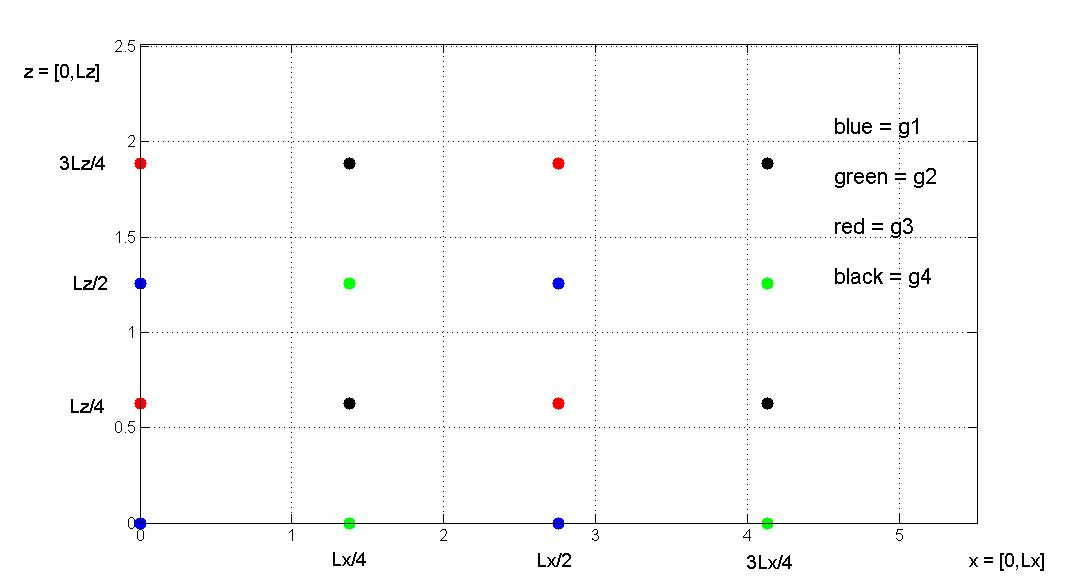
\includegraphics[width=0.95\textwidth]{stags7_26.jpg}
  \caption{
   Sets of possible \stagp s. If one of the $g_i$ symmetries is
   possessed, the velocity field will have \stagp s of the color
   corresponding to that symmetry.
   }
  \label{fig:stags7_26}
 \end{figure}



\subsection{Any nontrivial \stagp\ has a partner, symmetric about another {\stagp}}
% was {Proof that any new \stagp\ must have a partner, symmetric about one of the previously known {\stagp}s}

Though our symmetry arguments do not determine whether or not there may exist \emph{additional} {\stagp}s which are not forced by the $g_i$ symmetries in the preceding section, we can in fact that show that for Eulerian equilibria which exist in one of the flow-invariant subspaces that contains a $g_i$-symmetry (for example, $S$ has $g_3$ symmetry and $S_8$ has both $g_2$ and $g_3$ symmetry), any additional nontrivial {\stagp}s that exist must occur in symmetric pairs centered around the other known {\stagp}s.

Consider one of the Eulerian equilibria in the $S$-invariant subspace, such as {\tEQtwo}. Again, the
 action of $s_3 \in S$ on velocity fields gives:
 \beq    s_3 \, [u, v, w](x,y,z) = [-u,-v,-w](-x,\, -y,\, -z+L_z/2)\nnu\, .
 \eeq
 If $(x_{_{SP}},y_{_{SP}},z_{_{SP}})$ is a \stagp, $[u, v,
 w](x_{_{SP}},y_{_{SP}},z_{_{SP}}) = [0,0,0]$, then
 \bea s_3 \, [u, v, w](x_{_{SP}},y_{_{SP}},z_{_{SP}}) &=& [-u,-v,-w](-x_{_{SP}},\, -y_{_{SP}},\, -z_{_{SP}}+L_z/2) \nnu\, \\
 &=& [0,0,0](-x_{_{SP}},\, -y_{_{SP}},\, -z_{_{SP}}+L_z/2) .
 \eea
 Thus $(-x_{_{SP}},\, -y_{_{SP}},\, -z_{_{SP}}+L_z/2)$ is also a \stagp.

We may parameterize a line passing through two points 
$(x_{1}, y_{1}, z_{1}),(x_{2}, y_{2}, z_{2})$
 as
 \bea
  x &=& x_{1} + (x_{2} - x_{1})t \continue
  y &=& y_{1} + (y_{2} - y_{1})t \continue
  z &=& z_{1} + (z_{2} - z_{1})t \continue
  t &\in (-\infty,\infty) .
 \eea

 Using the two stagnation points $(x_{_{SP}},y_{_{SP}},z_{_{SP}})$ and $(-x_{_{SP}},-y_{_{SP}},-z_{_{SP}} + L_z/2)$ this becomes
 
 \bea
  x &=& x_{_{SP}}(1-2t) \continue
  y &=& y_{_{SP}}(1-2t) \continue
  z &=& z_{_{SP}}(1-2t) + \frac{L_{z}}{2} t .
 \eea
When $t = 1/2$ this system returns $(x,y,z) = (0,0,L_{z}/4)$, showing 
that \tSP{3} lies on the line between these two \stagp s, halfway in 
between them. 

If we invoke the box periodicities: $x = x + L_{x}$, $z = z + L_{z}$, it 
is easy to show that this pair of {\stagp}s is also symmetric about any 
of \tSP{1}--\tSP{4}. For example, consider the translation $\mathbf{x = x + L_{x}}$: \\

 \noindent $(x_{_{SP}},y_{_{SP}},z_{_{SP}})$ is a \stagp\ $\Rightarrow$
 $(-x_{_{SP}}+L_{x},-y_{_{SP}},z_{_{SP}}+L_{z}/2)$ a \stagp.
 \bea
  x &=& x_{_{SP}}(1-2t) + L_{x}t \continue
  y &=& y_{_{SP}}(1-2t) \continue
  z &=& z_{_{SP}}(1-2t) + \frac{L_{z}}{2} t .
 \eea
When $t = 1/2$ this returns $(x,y,z) = (L_{x}/2,0,L_{z}/4)$, so that the 
new stagnation points lie symmetrically on a line passing through \tSP{1}. 

For an Eulerian equilibrium invariant under $S_8$, such as {\tEQeight}, existence of 
any additional nontrivial {\stagp} will then imply \emph{two} 
additional {\stagp}s, based on the action of $g_2$ and $g_3$. 
 If $(x_{_{SP}},y_{_{SP}},z_{_{SP}})$ is a \stagp, then  
 $(-x_{_{SP}},\, -y_{_{SP}},\, -z_{_{SP}}+L_z/2)$ and 
 $(-x_{_{SP}} + L_x/2,\, -y_{_{SP}},\, -z_{_{SP}})$ are also \stagp s. 

We will investigate numerical methods to determine the possible existence 
of any nontrivial {\stagp}s. In fact for {\tEQtwo}, as we show in the next 
section, we do find such a point and its symmetric partner. These 
additional {\stagp}s are critical for understanding the flow dynamics in 
the Eulerian equilibrium field, as their stable and unstable manifolds provide us 
with an outline of the overall dynamics. 

